\documentclass[landscape,final,a0paper,fontscale=0.285]{baposter}
\usepackage{tkz-graph}
\usetikzlibrary{shapes}
\usepackage{amsmath, amsthm, amssymb}
\usepackage{calc}
\usepackage{amssymb}
\usepackage{relsize}
\usepackage{multirow}
\usepackage{rotating}
\usepackage{bm}
\usepackage{url}
\usepackage{enumitem}

\usepackage{graphicx}
\usepackage{multicol}

%\usepackage{times}
%\usepackage{helvet}
%\usepackage{bookman}
\usepackage{palatino}

\newcommand{\captionfont}{\footnotesize}

\usetikzlibrary{calc}

\newcommand{\SET}[1]  {\ensuremath{\mathcal{#1}}}
\newcommand{\MAT}[1]  {\ensuremath{\boldsymbol{#1}}}
\newcommand{\VEC}[1]  {\ensuremath{\boldsymbol{#1}}}
\newcommand{\Video}{\SET{V}}
\newcommand{\video}{\VEC{f}}
\newcommand{\track}{x}
\newcommand{\Track}{\SET T}
\newcommand{\LMs}{\SET L}
\newcommand{\lm}{l}
\newcommand{\PosE}{\SET P}
\newcommand{\posE}{\VEC p}
\newcommand{\negE}{\VEC n}
\newcommand{\NegE}{\SET N}
\newcommand{\Occluded}{\SET O}
\newcommand{\occluded}{o}


\makeatletter
\newtheorem*{rep@theorem}{\rep@title}
\newcommand{\newreptheorem}[2]{
\newenvironment{rep#1}[1]{
 \def\rep@title{#2 \ref{##1}}
 \begin{rep@theorem}}
 {\end{rep@theorem}}}
\makeatother

\theoremstyle{plain}
\newtheorem{thm}{Theorem}
\newreptheorem{thm}{Theorem}
\newtheorem{prop}[thm]{Proposition}
\newtheorem*{LLL}{Lov{\'a}sz Local Lemma}
\newreptheorem{prop}{Proposition}
\newtheorem{lem}[thm]{Lemma}
\newreptheorem{lem}{Lemma}
\newtheorem{conjecture}[thm]{Conjecture}
\newreptheorem{conjecture}{Conjecture}
\newtheorem{cor}[thm]{Corollary}
\newreptheorem{cor}{Corollary}
\newtheorem{prob}[thm]{Problem}
\theoremstyle{definition}
\newtheorem{defn}{Definition}
\theoremstyle{remark}
\newtheorem*{remark}{Remark}
\newtheorem{example}{Example}
\newtheorem*{question}{Question}
\newtheorem*{observation}{Observation}

\newcommand{\fancy}[1]{\mathcal{#1}}
\newcommand{\C}[1]{\fancy{C}_{#1}}
\newcommand{\IN}{\mathbb{N}}
\newcommand{\IR}{\mathbb{R}}
\newcommand{\G}{\fancy{G}}
\newcommand{\CC}{\fancy{C}}
\newcommand{\D}{\fancy{D}}

\newcommand{\inj}{\hookrightarrow}
\newcommand{\surj}{\twoheadrightarrow}

\newcommand{\set}[1]{\left\{ #1 \right\}}
\newcommand{\setb}[3]{\left\{ #1 \in #2 \mid #3 \right\}}
\newcommand{\setbs}[2]{\left\{ #1 \mid #2 \right\}}
\newcommand{\card}[1]{\left|#1\right|}
\newcommand{\size}[1]{\left\Vert#1\right\Vert}
\newcommand{\ceil}[1]{\left\lceil#1\right\rceil}
\newcommand{\floor}[1]{\left\lfloor#1\right\rfloor}
\newcommand{\func}[3]{#1\colon #2 \rightarrow #3}
\newcommand{\funcinj}[3]{#1\colon #2 \inj #3}
\newcommand{\funcsurj}[3]{#1\colon #2 \surj #3}
\newcommand{\irange}[1]{\left[#1\right]}
\newcommand{\join}[2]{#1 \mbox{\hspace{2 pt}$\ast$\hspace{2 pt}} #2}
\newcommand{\djunion}[2]{#1 \mbox{\hspace{2 pt}$+$\hspace{2 pt}} #2}
\newcommand{\parens}[1]{\left( #1 \right)}
\newcommand{\brackets}[1]{\left[ #1 \right]}
\newcommand{\DefinedAs}{\mathrel{\mathop:}=}
\newcommand{\im}{\operatorname{im}}
\newcommand{\ex}{\operatorname{E}}

\setlength{\columnsep}{1.5em}
\setlength{\columnseprule}{0mm}

\begin{document}

%\definecolor{lightblue}{cmyk}{0.83,0.24,0,0.12}
\definecolor{lightblue}{rgb}{0.145,0.6666,1}


\hyphenation{resolution occlusions}
%%
\begin{poster}%
  % Poster Options
  {
  % Show grid to help with alignment
  grid=false,
  % Column spacing
  colspacing=1em,
  % Color style
  bgColorOne=white,
  bgColorTwo=white,
  borderColor=lightblue,
  headerColorOne=black,
  headerColorTwo=lightblue,
  headerFontColor=white,
  boxColorOne=white,
  boxColorTwo=lightblue,
  % Format of textbox
  textborder=roundedleft,
  % Format of text header
  eyecatcher=true,
  headerborder=closed,
  headerheight=0.14\textheight,
%  textfont=\sc, An example of changing the text font
  headershape=roundedright,
  headershade=shadelr,
  headerfont=\bf\textsc, %Sans Serif
  textfont={\setlength{\parindent}{1.5em}},
  boxshade=plain,
%  background=shade-tb,
  background=plain,
  linewidth=1pt,
columns=4
  }
  {}
  {\bf\textsc{List coloring with large maximum degree}\vspace{0.5em}}
  {\textsc{Landon Rabern}\\School of Mathematical and Statistical Sciences, Arizona State University\\ Joint work with H.A. Kierstead}

\headerbox{A Prison Conjecture}{name=BK,column=0,row=0}{
\noindent Suppose you are a warden in a prison with eight large cells.  You need to put
all the prisoners into the cells, but to prevent fighting you cannot put
a pair of prisoners that have fought before into the same cell.  Each prisoner in
the prison has fought with at most nine other prisoners.  Under what conditions can you complete your task?

\begin{conjecture}[Borodin and Kostochka 1977 \cite{borodin1977upper}]
You can complete your task as long as there is no group of nine prisoners who have mutually fought one another.
\end{conjecture}

This problem can be modeled by a \emph{graph} where the prisoners are the \emph{vertices} and there is an \emph{edge} between each pair of prisoners who have fought each other.  The minimum number of cells that can be used corresponds to the \emph{chromatic number} $\chi$ and the most experienced fighter has fought with the \emph{maximum degree} $\Delta$ others.  A group of prisoners who have mutually fought one another form a \emph{clique}.  In this parlance, the conjecture says that a graph with $\Delta = 9$ has $\chi \leq \Delta - 1$ if it doesn't contain a clique on $\Delta$ vertices.  If true, it follows (see \cite{kostochkaRussian}, \cite{rabernhitting} and \cite{king2011hitting}) that the same result holds for all $\Delta \geq 9$.  For $\Delta = 8$, the conjecture fails due to the following example.

 \begin{center}
\begin{figure}[htb]
\centering
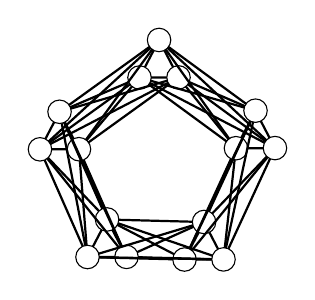
\begin{tikzpicture}[scale = 10]
\tikzstyle{VertexStyle}=[shape = circle,	
								 minimum size = 1pt,
								 inner sep = 3pt,
                         draw]
\Vertex[x = 0.257401078939438, y = 0.729450404644012, L = \tiny {}]{v0}
\Vertex[x = 0.232565611600876, y = 0.681758105754852, L = \tiny {}]{v1}
\Vertex[x = 0.282104313373566, y = 0.681911885738373, L = \tiny {}]{v2}
\Vertex[x = 0.383801102638245, y = 0.820650428533554, L = \tiny {}]{v3}
\Vertex[x = 0.358965694904327, y = 0.772958129644394, L = \tiny {}]{v4}
\Vertex[x = 0.40850430727005, y = 0.773111909627914, L = \tiny {}]{v5}
\Vertex[x = 0.506290018558502, y = 0.730872631072998, L = \tiny {}]{v6}
\Vertex[x = 0.48145455121994, y = 0.683180332183838, L = \tiny {}]{v7}
\Vertex[x = 0.530993163585663, y = 0.683334112167358, L = \tiny {}]{v8}
\Vertex[x = 0.440956592559814, y = 0.589494824409485, L = \tiny {}]{v9}
\Vertex[x = 0.416121125221252, y = 0.541802525520325, L = \tiny {}]{v10}
\Vertex[x = 0.46565979719162, y = 0.541956305503845, L = \tiny {}]{v11}
\Vertex[x = 0.317756593227386, y = 0.592694818973541, L = \tiny {}]{v12}
\Vertex[x = 0.292921125888824, y = 0.545002520084381, L = \tiny {}]{v13}
\Vertex[x = 0.342459797859192, y = 0.545156300067902, L = \tiny {}]{v14}
\Edge[](v2)(v1)
\Edge[](v2)(v0)
\Edge[](v1)(v0)
\Edge[](v4)(v3)
\Edge[](v5)(v3)
\Edge[](v5)(v4)
\Edge[](v7)(v6)
\Edge[](v8)(v6)
\Edge[](v8)(v7)
\Edge[](v10)(v9)
\Edge[](v11)(v9)
\Edge[](v11)(v10)
\Edge[](v13)(v12)
\Edge[](v14)(v12)
\Edge[](v14)(v13)
\Edge[](v3)(v0)
\Edge[](v4)(v0)
\Edge[](v5)(v0)
\Edge[](v3)(v2)
\Edge[](v4)(v2)
\Edge[](v5)(v2)
\Edge[](v3)(v1)
\Edge[](v4)(v1)
\Edge[](v5)(v1)
\Edge[](v3)(v6)
\Edge[](v4)(v6)
\Edge[](v5)(v6)
\Edge[](v3)(v7)
\Edge[](v4)(v7)
\Edge[](v5)(v7)
\Edge[](v3)(v8)
\Edge[](v4)(v8)
\Edge[](v5)(v8)
\Edge[](v6)(v9)
\Edge[](v7)(v9)
\Edge[](v8)(v9)
\Edge[](v6)(v11)
\Edge[](v7)(v11)
\Edge[](v8)(v11)
\Edge[](v6)(v10)
\Edge[](v7)(v10)
\Edge[](v8)(v10)
\Edge[](v12)(v10)
\Edge[](v13)(v10)
\Edge[](v14)(v10)
\Edge[](v12)(v9)
\Edge[](v13)(v9)
\Edge[](v14)(v9)
\Edge[](v12)(v11)
\Edge[](v13)(v11)
\Edge[](v14)(v11)
\Edge[](v12)(v2)
\Edge[](v13)(v2)
\Edge[](v14)(v2)
\Edge[](v12)(v1)
\Edge[](v13)(v1)
\Edge[](v14)(v1)
\Edge[](v12)(v0)
\Edge[](v13)(v0)
\Edge[](v14)(v0)
\end{tikzpicture}
\caption{$M_8$: A $C_5$ with vertices blown-up to triangles.}
\label{fig:M_8}
\end{figure}

\end{center}

In 1999, Reed \cite{reed1999strengthening} proved the conjecture for $\Delta \geq 10^{14}$ using probabilistic methods.  Using a similar method, we prove the same result for list coloring with $\Delta \geq 10^{10^{15}}$.
 }

\headerbox{Picky Prisoners}{name=listcolor,column=1, row=0}{
\noindent Now suppose your prison has infinitely many cells, but each prisoner has a list of the $\Delta-1$ cells he can occupy.  When, for every possible assignment of lists to the prisoners, can you put the prisoners into the cells so that each is in a cell on his list and no former rivals are in the same cell?  This is the \emph{list coloring} problem and we write $\chi_l$ for the minimum prisoner list size that will work.  In graph theory parlance the big conjecture here says that a graph with $\Delta \geq 9$ has $\chi_l \leq \Delta - 1$ if it doesn't contain a clique on $\Delta$ vertices.  We prove this for very large $\Delta$.

\begin{thm}
Every graph with $\Delta \geq 10^{10^{15}}$ has $\chi_l \leq \Delta-1$ if it doesn't contain a clique on $\Delta$ vertices.
\end{thm}
  }

\headerbox{Proceed Randomly}{name=random,column=1,below=listcolor}{
\noindent We analyze the following simple random process.
\begin{itemize}[noitemsep,nolistsep]
\item put each prisoner into a randomly chosen cell from his list
\item send all prisoners who were put in a cell with a former rival to the yard
\end{itemize}

\noindent We show that with nonzero probability it is possible to put the prisoners in the yard back into cells in a way that works.  It follows that there is at least one way to complete the task.
}
\headerbox{Safe Prisoners}{name=safe,column=1,below=random}{
\noindent Suppose Atticus is a prisoner who was sent to the yard after the random cell selection.  If there are two different cells which each contain at least two of Atticus' former rivals, then no matter how the rest of the prisoners are put back in the cells, Atticus will have a legal cell available.  Similarly, if there are two different cells, neither of which are on Atticus' list, each containing one of Atticus' former rivals, then a legal cell will always remain for Atticus.  If either of these two situations or a combination of the two occur, then Atticus is \emph{safe}.

\noindent We don't need to worry about safe prisoners, they can just hang out in the yard until we have placed the rest.
}
\headerbox{A Structural Decomposition}{name=structure,column=2,row=0}{
\noindent The prisoners in no big cliques can be shown to be safe with very high probability.  The prisoners in big cliques need special care.  Basically, we show that each prisoner that is in a big clique is in exactly one big clique.  To prove the decomposition, we use many small graphs that were proved to be reducible configurations in \cite{cranstonrabernapriori}.
}

\headerbox{Handling Big Cliques}{name=handling,column=2,below=structure}{
\noindent With the above structural decomposition, we may proceed as follows. We show that with high probability each big clique has two safe prisoners in the yard.  By leaving these two prisoners in the yard until the rest of the prisoners in their clique are placed, each other prisoner will always have a legal cell available.
}

\headerbox{Five Bad Events}{name=bad,column=2,below=handling}{
\noindent We've mentioned two bad events so far: a prisoner in no big clique that isn't safe and a big clique that doesn't have two safe prisoners in the yard.  In fact, to get all the details right, there are three other bad events our analysis uses.  We show that each of these events happens with low probability.  Since the events are not independent, this is not enough to conclude that the probability that none of the events happen is nonzero.  To reach this conclusion we apply the Lov{\'a}sz Local Lemma.

\begin{LLL}
If there is a collection of events each occuring with probability at most $p$ such that each event is independent of all but at most $d$ others and $pd \leq \frac14$, then the probability that none of the events happen is nonzero.
\end{LLL}
}

\headerbox{Future Directions}{name=future,column=3,row=0}{
\noindent If we add the assumption that none of the
prisoners who have fought with $\Delta$ others have fought with each other, then in the regular coloring case we can complete our task when $\Delta \geq 6$ so long as there is no clique of $\Delta$ prisoners (see \cite{kierstead2009ore}, \cite{rabern2010a}, \cite{krs_one}, \cite{rabern2012partitioning} and \cite{kostochka2012ore}).  What of the same question for list coloring?

The result proved here was independently proved by Choi and Reed, our merged proof improving the bound on $\Delta$ to $\Delta \geq 10^{20}$ will appear in \cite{BKListLarge}.
   \vspace{0.3em}
  }
  \headerbox{References}{name=references,column=3, below=future}{
    \scriptsize
    \renewcommand{\section}[2]{}
    \bibliographystyle{amsplain}
	\bibliography{GraphColoring}
   \vspace{0.3em}
  }



\end{poster}

\end{document}
